\chapter{Introduzione alla fisica delle particelle e il mesone $D^{*+}$ }

\section{La fisica subnucleare e il Modello Standard}
A partire dall'esperimento di Rutherford nel 1909 si è sviluppato l'ambito della fisica nucleare e subnucleare. Per quanto riguarda la fisica delle particelle, il modello che attualmente ne descrive i fondamenti è il \textit{Modello Standard}. Le particelle fondamentali sono divise tra fermioni e bosoni. Ogni particella riportata in figura \ref{fig:ModelloStandard} ha la sua antiparticella (ad eccezione del fotone che è l'antiparticella di se stesso). 

    \begin{figure}[htbp]
        \centering
        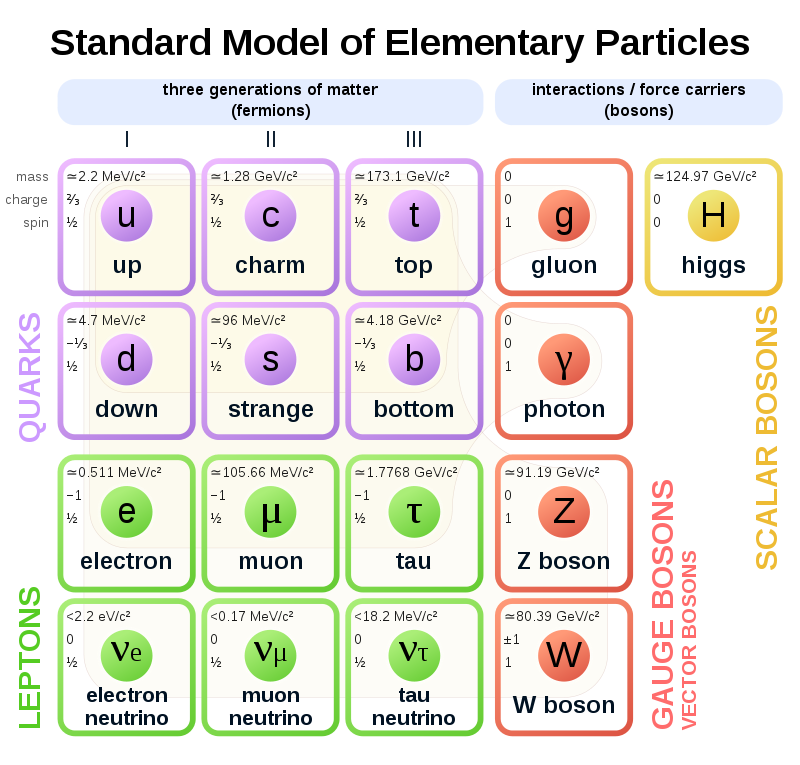
\includegraphics[width=0.65\linewidth]{introParticelle/ModelloStandard.png}
        \caption{Schema del Modello Standard}
        \label{fig:ModelloStandard}
    \end{figure}
    
Nella parte sinistra della figura \ref{fig:ModelloStandard} si trovano i \textit{fermioni} divisi tra quark e leptoni. Sono divisi in tre generazioni ordinate in base a valori di massa crescente, pertanto più è alto l'ordine della generazione più rare e instabili sono le particelle corrispondenti. I quark sono contraddistinti dal sapore (ad esempio: top, down, charm e così via) e non possono esistere mai da soli ma formano solitamente barioni (3 quark) o mesoni (coppie di un quark e un anti-quark).Le particelle non elementari così formate possono trovarsi nel loro stato fondamentale o in stati eccitati, in questo ultimo caso si indicano solitamente con l'apice $^*$. \cite{libro_nucleare}
Nella parte destra della figura \ref{fig:ModelloStandard} si trovano i \textit{bosoni} divisi tra i bosoni di Gauge, che sono i trasportatori delle forze fondamentali e il bosone di Higgs, che è l'unico bosone scalare (di spin 0) rivelato per la prima volta nel 2012 al Cern.

    \subsection{I decadimenti}
    Le particelle possono essere più o meno stabili, in caso di particelle instabili queste tendono a decadere. Il decadimento può essere di tipo forte, di tipo debole o di tipo elettromagnetico. I decadimenti devono rispettare varie leggi di conservazione, in particolare il decadimento debole è l'unico che permette alla particella di cambiare il proprio sapore. Alcune particelle possono decadere secondo più vie. Ciascuna di esse è caratterizzata dal branching ratio (BR), che consiste nella percentuale di probabilità di verificarsi di quel decadimento specifico rispetto a tutti quelli possibili.
    \\La particella che decade ha una vita media $\tau$, chiamata anche tempo caratteristico del decadimento. Da questo si può ricavare il cammino medio come: $l = v \tau$, nel caso di particelle altamente relativistiche di può considerare $l = c \tau$. 
    
    
\section{QCD e QGP}
La teoria che descrive l'interazione forte tra i quark è la \textit{Quantum Chromo Dynamics} (QCD). I quark sono caratterizzati da una carica di colore, che ha tre diversi stati, solitamente individuati come rosso, blu e verde. L'interazione tra quark avviene attraverso i gluoni, anche questi portatori di carica di colore. Inoltre, i gluoni possono interagire anche fra di loro scambiando altri gluoni. Uno degli effetti della QCD è il cosidetto \textit{confinamento}, questo prevede che non potendo esistere particelle colorate, i quark siano "confinati" all'interno di strutture (come barioni e mesoni) con colore neutro e, se si tenta di isolare un quark singolo, l'effetto è quello di aumentare la forza che lo tiene legato all'altro quark. Al contrario se i quark si trovano molto vicini tra di loro si ottiene la "libertà asintotica", ovvero la forza che tiene legati i due quark diminuisce ottenendo uno stato in cui le particelle sono quasi libere. \cite{libro_nucleare}
\\Di conseguenza, la materia ad altissime temperature o densità di energia attraversa un cambiamento di stato, passando dallo stato in cui i quark sono confinati ad uno in cui i quark e i gluoni sono liberi di muoversi in spazi molto più grandi rispetto alle dimensioni degli adroni \footnote{Un adrone è una particella formata da quark, come ad esempio mesoni e barioni}. Questo stato è chiamato \textit{Quark Gluon Plasma} (QGP). \cite{QCD} 

\begin{figure}[htbp]
        \centering
        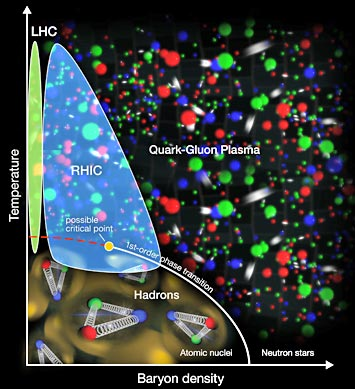
\includegraphics[width=0.5\linewidth]{introParticelle/DiagrammaFaseQGP2.jpg}
        \caption{ Diagramma di fase schematico della materia fortemente interagente, in cui si mostra la transizione di fase verso il QGP}
        \label{fig:DiagrammaFaseQCD}
    \end{figure}
    
    
Per descrivere i cambiamenti di stato della materia che interagisce in modo forte si utilizza un diagramma di fase che riporta sugli assi la temperatura e il potenziale chimico-barionico $\mu_B$. Quest'ultimo è definito come la quantità di energia necessaria per aumentare di un'unità il numero barionico, pertanto è direttamente correlato alla densità barionica.
\\Per poter studiare il QGP vengono condotti esperimenti quali RHIC (Relativstic Heavy-Ion Collider) e LHC, che come si vede in figura \ref{fig:DiagrammaFaseQCD} creano nelle loro collisioni condizioni tali che la materia sia nello stato di Quark Gluon Plasma. 
\\Il tempo in cui esiste il QGP ad ALICE è di circa $10 fm/c$ ($t \simeq 10^{-23}$s) \cite{QCD2}, pertanto è impossibile studiarlo direttamente, in quanto le particelle, in così poco tempo, non arriverebbero neanche ai primi rivelatori. Gli adroni composti da quark di tipo charm o beauty vengono solitamente utilizzati per studiare il QGP. Questo perchè i quark pesanti vengono prodotti poco dopo la collisione tra nucleoni ($\leq 0.1 fm/c \simeq 0.3 10^{-24}$s) in tempi minori rispetto a quelli della formazione del QGP ($\simeq 0.3 - 1.5 fm/c \simeq 10^{-24} - 0.5 10^{-23}$s). Inoltre, i quark pesanti hanno sia un tasso di annichilazione che di produzione durante la fase di QGP che ci si aspetta sia trascurabile. Perciò i quark pesanti preservano la loro identità mentre attraversano il Quark Gluon Plasma e possono essere studiati per ricavare informazioni sul QGP. \cite{tesi_barbano}


\section{Il mesone $D^{*+}$} \label{mesoneD}
Nel corso di questa tesi si prenderà in esame il mesone $D^{*+}$, pertanto ne vediamo brevemente le caratteristiche e i principali modi di decadimento. Il mesone $D^{+}$ è formato da un quark charm $c$ e un quark anti-down $\overline{d}$, il mesone $D^{*+}$ ne è uno stato eccitato, in cui il momento angolare totale è diverso da 0. Nei mesoni $D$ solitamente il quark charm decade in un quark strange $s$, pertanto spesso la particella decade in un Kaone $K$. 
\\L'esperimento ALICE ha studiato la produzione dei mesoni charm e e beauty fin dal primo periodo di presa dati di LHC. I mesoni $D^0$, $D^+$, $D^{*+}$, $D_s^+$  sono stati studiati in un intervallo di momento trasverso $p_T$ da 1 a 24 $GeV/c$.  \cite{mesoniD}
\\La $D^{*+}$ ha una massa di $2010.26 \pm 0.05$ $MeV/c^2$ e tempo di vita media $ \tau = (7.89 \pm 0.11) {10^{-21}}$s. Il modo di decadimento principale $D^{*+} \rightarrow D^0 + \pi^+ $ ha un BR = $67.7$ $\% $ ed è proprio il decadimento che si è usato per l'analisi dati di questa tesi. La $D^0$ ha massa $ 1864.83 \pm 0.05 $ $MeV/c^2$, decade $D^0 \rightarrow K^- \pi^+$ con un BR = $3.89$ $\%$ ed ha una vita media di $(410.1 \pm 1.5 ) 10^{-15} s $.
\\La $D^{*+}$ può decadere anche come $D^+$ e $\pi^0$ con un BR = $30.7$ $\%$. \cite{PDG}

    \begin{figure}[htbp]
        \centering
        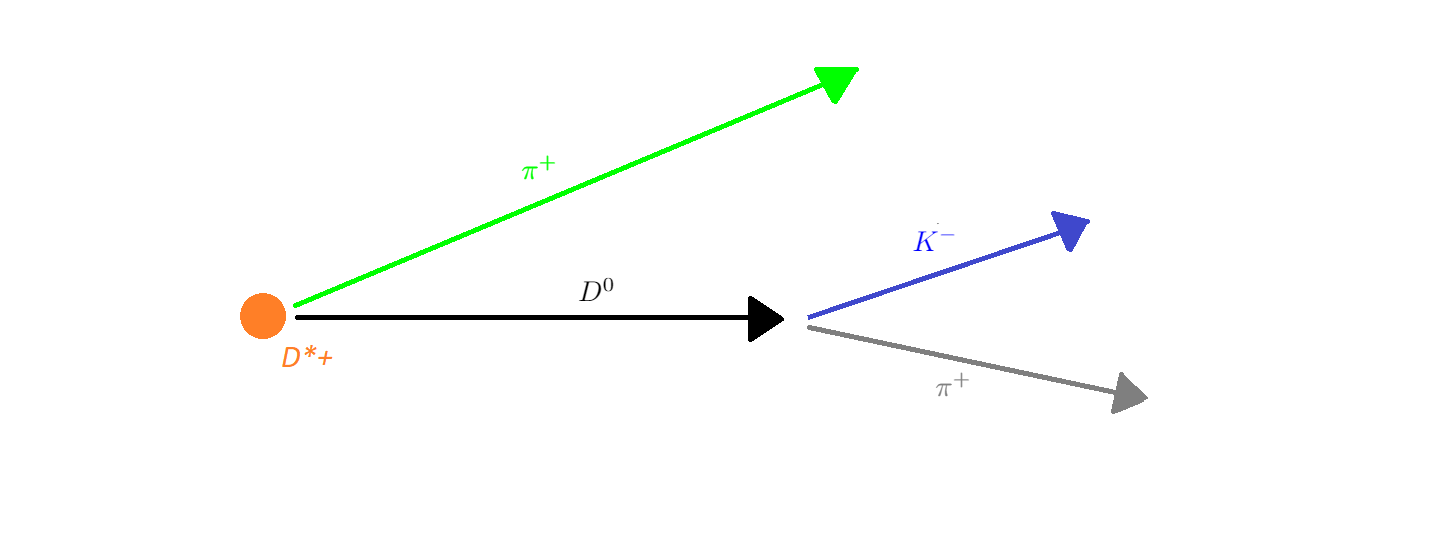
\includegraphics[width=1.0\linewidth]{introParticelle/decadimentoD.png}
        \caption{ Schema del decadimento del mesone $D^{*+}$}
        \label{fig:decadimentoD}
    \end{figure}









